% !BIB TS-program = biber

\RequirePackage[l2tabu,orthodox]{nag}

% TODO: decide if one-sided/two-sided
%\documentclass[headsepline,footsepline,footinclude=false,fontsize=11pt,paper=a4,listof=totoc,bibliography=totoc,BCOR=12mm,DIV=12]{scrbook} % two-sided
\documentclass[headsepline,footsepline,footinclude=false,oneside,fontsize=11pt,paper=a4,listof=totoc,bibliography=totoc]{scrbook} % one-sided

\PassOptionsToPackage{table,svgnames,dvipsnames}{xcolor}

\usepackage[utf8]{inputenc}
\usepackage[T1]{fontenc}
\usepackage[sc]{mathpazo}
\usepackage[american]{babel}
\usepackage[autostyle]{csquotes}
\usepackage[%
  backend=biber,
  url=true,
  sorting=none,
  style=numeric-comp,
  maxnames=4,
  minnames=3,
  maxbibnames=99,
  giveninits,
  uniquename=init]{biblatex}
\usepackage{graphicx}
\usepackage{subcaption}
\usepackage{tabularray}
\UseTblrLibrary{booktabs}
\usepackage{mathtools}
\usepackage{scrhack} % necessary for listings package
\usepackage{listings}
\usepackage{lstautogobble}
\usepackage{tikz}
\usepackage{pgfplots}
\usepackage{pgfplotstable}
\usepackage{booktabs}
\usepackage[final]{microtype}
\usepackage{caption}
\usepackage[printonlyused]{acronym}
\usepackage[hidelinks]{hyperref} % hidelinks removes colored boxes around references and links
\AtBeginDocument{%
	\hypersetup{
		pdftitle=\getTitle,
		pdfauthor=\getAuthor,
	}
}
\usepackage{ifthen}

\addto\extrasamerican{
	\def\lstnumberautorefname{Line}
	\def\chapterautorefname{Chapter}
	\def\sectionautorefname{Section}
	\def\subsectionautorefname{Subsection}
	\def\subsubsectionautorefname{Subsubsection}
}

\addto\extrasngerman{
	\def\lstnumberautorefname{Zeile}
}

% Themes
\ifthenelse{\equal{\detokenize{dark}}{\jobname}}{%
  % Dark theme
  \newcommand{\bg}{black} % background
  \newcommand{\fg}{white} % foreground
  \usepackage[pagecolor=\bg]{pagecolor}
  \color{\fg}
}{%
  % Light theme
  \newcommand{\bg}{white} % background
  \newcommand{\fg}{black} % foreground
}

\bibliography{bibliography}

\setkomafont{disposition}{\normalfont\bfseries} % use serif font for headings
\linespread{1.05} % adjust line spread for mathpazo font

% Add table of contents to PDF bookmarks
\BeforeTOCHead[toc]{{\cleardoublepage\pdfbookmark[0]{\contentsname}{toc}}}

% Define TUM corporate design colors
% Taken from http://portal.mytum.de/corporatedesign/index_print/vorlagen/index_farben
\definecolor{TUMBlue}{HTML}{0065BD}
\definecolor{TUMSecondaryBlue}{HTML}{005293}
\definecolor{TUMSecondaryBlue2}{HTML}{003359}
\definecolor{TUMBlack}{HTML}{000000}
\definecolor{TUMWhite}{HTML}{FFFFFF}
\definecolor{TUMDarkGray}{HTML}{333333}
\definecolor{TUMGray}{HTML}{808080}
\definecolor{TUMLightGray}{HTML}{CCCCC6}
\definecolor{TUMAccentGray}{HTML}{DAD7CB}
\definecolor{TUMAccentOrange}{HTML}{E37222}  % Software
\definecolor{TUMAccentGreen}{HTML}{A2AD00}
\definecolor{TUMAccentLightBlue}{HTML}{98C6EA}
\definecolor{TUMAccentBlue}{HTML}{64A0C8}    % Hardware

% Settings for pgfplots
\pgfplotsset{compat=newest}
\pgfplotsset{
  % For available color names, see http://www.latextemplates.com/svgnames-colors
  cycle list={TUMBlue\\TUMAccentOrange\\TUMAccentGreen\\TUMSecondaryBlue2\\TUMDarkGray\\},
}

% Settings for lstlistings
\lstset{%
  basicstyle=\ttfamily,
  columns=fullflexible,
  autogobble,
  keywordstyle=\bfseries\color{TUMBlue},
  stringstyle=\color{TUMAccentGreen},
  captionpos=b
}


\newcommand*{\getUniversity}{Technische Universität München}
\newcommand*{\getFaculty}{Informatics}
\newcommand*{\getDegree}{Informatics}
\newcommand*{\getSchool}{Computation, Information and Technology}
\newcommand*{\getTitle}{Establishing trust in an updatable fTPM using remote
attestation}
\newcommand*{\getTitleGer}{Herstellung von Vertrauen in ein aktualisierbares fTPM durch
Remote Attestierung}
\newcommand*{\getAuthor}{Andreas Korb}
\newcommand*{\getDoctype}{Master's Thesis}
\newcommand*{\getSupervisor}{Prof. Claudia Eckert}
\newcommand*{\getAdvisor}{Albert Stark}
\newcommand*{\getSubmissionDate}{15.11.2023}
\newcommand*{\getSubmissionLocation}{Munich}

\begin{document}

% Set page numbering to avoid "destination with the same identifier has been already used" warning for cover page.
% (see https://en.wikibooks.org/wiki/LaTeX/Hyperlinks#Problems_with_Links_and_Pages).
\pagenumbering{alph}
\input{pages/cover}

\frontmatter{}

\begin{titlepage}
  \centering

  \IfFileExists{logos/tum-\fg.pdf}{%
    \includegraphics[height=20mm]{logos/tum-\fg.pdf}
  }{%
    \vspace*{20mm}
  }

  \vspace{5mm}
  {\huge\MakeUppercase{School of \getSchool{} --- \getFaculty{}} \par}

  \vspace{5mm}
  {\large\MakeUppercase{\getUniversity{}} \par}

  \vspace{20mm}
  {\Large \getDoctype{} in \getDegree{} \par}

  \vspace{15mm}
  {\huge\bfseries \getTitle{} \par}

  \vspace{10mm}
  {\huge\bfseries \foreignlanguage{ngerman}{\getTitleGer{}} \par}

  % TODO Verify whether setting 10mm instead of 15mm here is okay
  \vspace{10mm}
  \begin{tabular}{l l}
    Author:          & \getAuthor{}         \\
    Supervisor:      & \getSupervisor{}     \\
    Advisor:         & \getAdvisor{}        \\
    Submission Date: & \getSubmissionDate{} \\
  \end{tabular}

  \IfFileExists{logos/faculty-\fg.pdf}{%
    \vfill{}
    \includegraphics[height=20mm]{logos/faculty-\fg.pdf}
  }{}
\end{titlepage}

\thispagestyle{empty}
\vspace*{0.8\textheight}
\noindent
I confirm that this \MakeLowercase{\getDoctype{}} is my own work and I have documented all sources and material used.

\vspace{15mm}
\noindent
\getSubmissionLocation{}, \getSubmissionDate{} \hspace{\fill} \getAuthor{}

\cleardoublepage{}

\addcontentsline{toc}{chapter}{Acknowledgments}
\thispagestyle{empty}

\vspace*{20mm}

\begin{center}
    {\usekomafont{sectioning}\usekomafont{section} Acknowledgments}
\end{center}

\vspace{10mm}

I would like to take this opportunity to thank all those who have supported me in the preparation of this thesis.
My thanks go to my supervisor Prof.\ Dr.\ Claudia Eckert, who gave me the opportunity to write this thesis.
I would also like to express my special thanks to my advisors Albert Stark and Johannes Wiesböck, who patiently stood by my side and answered all my questions.
Without their help and support, this thesis would not have been possible, and I am sure they have helped me greatly to start my journey in the field of cyber security.
Last but not least, I would like to thank all my friends who have been patient and understanding during the writing of this thesis and who have sacrificed their time to proofread my work.


\cleardoublepage{}

\chapter{\abstractname}

Zero Trust is a cybersecurity paradigm in which a network, e.g., an enterprise network, is considered compromised.
Therefore, each device of every service request must be verified before the request is served.
This is made possible by remote attestation, which is enabled by TPMs, for example.
For that, they authenticate themselves by propagating their so-called endorsement certificate naming their manufacturer, who guarantees they conform to the TPM specification to ensure their security properties.
While this approach is sufficient for hardware TPMs as they are standalone chips, for firmware TPMs~(fTPM) it is assumed that the manufacturer of the fTPM is the same as that of all firmware components that were booted before the fTPM\@.
This is due to the fact that any previous firmware component can compromise the fTPM during loading.
The verifier in the remote attestation procedure lacks the ability of verifying the entire boot chain up to the fTPM\@.
We propose a remote attestation system that provides the verifier with this possibility.
To compensate for the lack of a hardware root of trust of an fTPM compared to a hardware TPM, we introduce DICE as the hardware root of trust.
The verifier only needs to trust the manufacturer of DICE, while every firmware component beyond is explicitly attested by passing their identities to the verifier.
The three benefits of our solution are that (i) the manufacturer of the fTPM and its preceding firmware components can be independent of each other, (ii) detection of modification of fTPM by remote verifier, and (iii) protection of the fTPM's data-at-rest.
% Explain (ii)
DICE measures the first firmware component, which is then repeated up to the fTPM\@.
These measurements are forwarded to the remote verifier, which can then detect potentially malicious changes to each measured component.
% Explain (iii)
The fTPM's data-at-rest is protected by binding it to the identity of the fTPM\@.
This means that the data of an fTPM is only accessible to the fTPM that created it as long as its identity does not change, which makes downgrade attacks and changes to the fTPM less attractive to attackers.

\microtypesetup{protrusion=false}
\tableofcontents{}
\microtypesetup{protrusion=true}

\mainmatter{}

%% !TeX root = ../main.tex
% Add the above to each chapter to make compiling the PDF easier in some editors.

\chapter{Template examples}

\section{Section}
Citation test~\parencite{latex}.

Acronyms must be added in \texttt{main.tex} and are referenced using macros. The first occurrence is automatically replaced with the long version of the acronym, while all subsequent usages use the abbreviation.

E.g. \texttt{\textbackslash ac\{TUM\}, \textbackslash ac\{TUM\}} $\Rightarrow$ \ac{TUM}, \ac{TUM}

For more details, see the documentation of the \texttt{acronym} package\footnote{\url{https://ctan.org/pkg/acronym}}.
\subsection{Subsection}

See~\autoref{tab:sample}, \autoref{fig:sample-drawing}, \autoref{fig:sample-plot}, \autoref{fig:sample-listing}.

\begin{table}[htpb]
  \caption[Example table]{An example for a simple table.}\label{tab:sample}
  \centering
  \begin{tabular}{l l l l}
    \toprule
      A & B & C & D \\
    \midrule
      1 & 2 & 1 & 2 \\
      2 & 3 & 2 & 3 \\
    \bottomrule
  \end{tabular}
\end{table}

\begin{figure}[htpb]
  \centering
  % This should probably go into a file in figures/
  \begin{tikzpicture}[node distance=3cm]
    \node (R0) {$R_1$};
    \node (R1) [right of=R0] {$R_2$};
    \node (R2) [below of=R1] {$R_4$};
    \node (R3) [below of=R0] {$R_3$};
    \node (R4) [right of=R1] {$R_5$};

    \path[every node]
      (R0) edge (R1)
      (R0) edge (R3)
      (R3) edge (R2)
      (R2) edge (R1)
      (R1) edge (R4);
  \end{tikzpicture}
  \caption[Example drawing]{An example for a simple drawing.}\label{fig:sample-drawing}
\end{figure}

\begin{figure}[htpb]
  \centering

  \pgfplotstableset{col sep=&, row sep=\\}
  % This should probably go into a file in data/
  \pgfplotstableread{
    a & b    \\
    1 & 1000 \\
    2 & 1500 \\
    3 & 1600 \\
  }\exampleA
  \pgfplotstableread{
    a & b    \\
    1 & 1200 \\
    2 & 800 \\
    3 & 1400 \\
  }\exampleB
  % This should probably go into a file in figures/
  \begin{tikzpicture}
    \begin{axis}[
        ymin=0,
        legend style={legend pos=south east},
        grid,
        thick,
        ylabel=Y,
        xlabel=X
      ]
      \addplot table[x=a, y=b]{\exampleA};
      \addlegendentry{Example A};
      \addplot table[x=a, y=b]{\exampleB};
      \addlegendentry{Example B};
    \end{axis}
  \end{tikzpicture}
  \caption[Example plot]{An example for a simple plot.}\label{fig:sample-plot}
\end{figure}

\begin{figure}[htpb]
  \centering
  \begin{tabular}{c}
  \begin{lstlisting}[language=SQL]
    SELECT * FROM tbl WHERE tbl.str = "str"
  \end{lstlisting}
  \end{tabular}
  \caption[Example listing]{An example for a source code listing.}\label{fig:sample-listing}
\end{figure}

% !TeX root = ../main.tex
% Add the above to each chapter to make compiling the PDF easier in some editors.

\chapter{Introduction}\label{chapter:introduction}

This chapter explains the problem we are addressing, why, a brief overview of our solution, and the attacks we are trying to fend off.

% nicht wissenschaftliche Teil, zero trust ist jetzt ein Ding, immer mehr embedded ohne TPM (z.B. Gartner Studien)

\section{Motivation}

% Which area this thesis is talking about (Zero Trust)

Modern trust relationships, such as Zero Trust~\cite{isaca2021}, require trustworthy platforms to reliably report their system state.
In such models, trust is no longer implicitly assumed, e.g., by the fact that a device is located within the boundaries of a company.
Instead, each device is considered compromised until proven otherwise on a per-request basis for resources (e.g., printers) and data access~\cite{Rose2020}.

% Primer on remote attestation

This is solved by remote attestation.
In the simplest case, there is a prover and a verifier, as depicted in \autoref{fig:ra_simple}.
The challenge is that the verifier observes nothing but bytes from the prover, and while a benign prover will tell the truth about its state, a compromised prover will lie about its state and claim a trustworthy one.
Therefore, the verifier must establish trust in a helper component on the prover's side.
In a typical setup, this component is immutable without the involvement of its manufacturer, which reveals itself to a verifier by signing and storing a certificate on the helper components supplied by it.
This allows the verifier to establish trust in the helper component by knowing its manufacturer.
Consequently, the component attests to the state of the prover's machine, from which the verifier can deduce whether the prover can be considered trustworthy.

\begin{figure}[htpb]
  \centering
  \includegraphics[width=0.5\linewidth]{figures/remote_attestation_process.pdf}
  \caption{Simplified remote attestation process.}\label{fig:ra_simple}
\end{figure}


% TPMs become more important

For example, this can be done with a \ac{TPM} on the prover's side. They rise in their deployments and importance, e.g., in 2013, the President's Council of Advisors on Science and Technology encouraged the adoption of TPMs~\cite{usa}, and Microsoft publicized that they require a TPM module for Windows~11 in 2021~\cite{win11req}.
They provide remote attestation mechanisms of system states, and their applications are still expanding beyond their traditional use cases. For example, they are used in anti-cheat software for games~\cite{valorant}.

% Short intro on why fTPMs were introduced (for weak devices, exactly our target platform)

A \ac{dTPM} increases cost and hardware complexity---especially for embedded platforms.
\Acp{fTPM} running in a \acp{TEE} can be used to provide similar security guarantees as a \ac{dTPM} chip.

% Why establishing trust in an fTPM is harder than in a dTPM

For a \ac{dTPM}, which consists of an independent hardware unit manufactured by a single manufacturer, it is sufficient to identify its manufacturer and understand their provided guarantees.
In contrast, an \ac{fTPM} runs atop other firmware components and is started later in the boot chain, making its security dependent on the underlying firmware stack.
Consequently, trust in an \ac{fTPM} depends on trusting the entire stack beneath it because its underlying firmware might alter or compromise the \ac{fTPM}.

% What's the difficulty of establishing trust in an fTPM?

However, while a TPM-compliant component provides an infrastructure with which trust in it can be established remotely, i.e., an endorsement (key) certificate~(EKcert), this does not represent the underlying firmware stack.

% How it currently works for fTPMs

Currently, this is solved by the manufacturer providing not only the fTPM, but also the entire underlying firmware stack.
Consequently, by establishing trust in the manufacturer of the fTPM, one can implicitly trust the underlying firmware by assuming they also originate from this manufacturer.
This is possible since, in the most general sense, one can derive from an endorsement certificate the endorser, i.e., manufacturer.
If the attester trusts the manufacturer and its provided guarantees, trust is established in its provided components.

\begin{figure}[htpb]
  \centering
  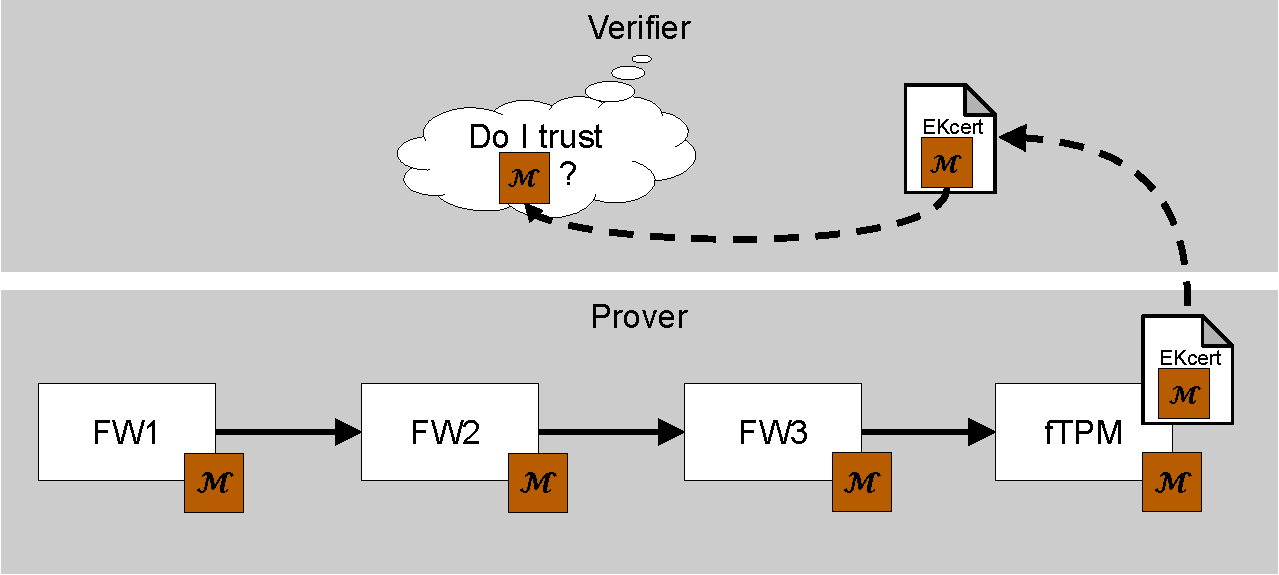
\includegraphics[width=1\linewidth]{figures/current_state.pdf}
  \caption{The naive process how a verifier establishes trust to an \ac{fTPM}, which is in fact done by trusting its manufacturer. The brown markers indicate a manufacturer. The firmware~(FW) and the fTPM were built by manufacturer \(\mathcal{M}\), and the EK certificate indicates this manufacturer.}\label{fig:current_state}
\end{figure}


This process is illustrated in figure \autoref{fig:current_state}.
The prover's box shows its boot chain, and the verifier's box shows how it evaluates the trustworthiness against the prover's boot chain.
The verifier trusts the entire firmware chain if it trusts the manufacturer of each component.
Note how the verifier must assume that the manufacturer of the firmware components is the same as that of the fTPM\@.
To the best of our knowledge, this is what manufacturers like Intel and AMD implement for their \acp{fTPM}, as confidence in their \acp{fTPM} is also only established through an EKcert~\cite{Ruan2014}.

% Summary with limitations

In summary, with the current approach, the endorser, usually a CPU manufacturer, provides the firmware up to the fTPM and guarantees the firmware is not modifiable by untrusted parties.
This enables trust in the other firmware components this manufacturer provided without knowing the firmware.
This approach is limited, as with this mechanism, independent verifiers have to unquestioningly trust the firmware manufacturer, drastically limiting trust relationships.

\section{Goal}

We establish an independently verifiable fTPM stack, rooted in a hardware root of trust, that can be leveraged in a Zero Trust environment with few hardware requirements and without compromising security.
This approach aims to break the requirement of the underlying firmware and the fTPM to originate from the same manufacturer by providing the exact firmware component identities to the verifier, such that it can decide whether they are trustworthy without relying on its manufacturer.
Instead, it is sufficient to trust the independent manufacturer of the hardware root of trust, which requires minimal assumptions, such as the absence of side-channel vulnerabilities.

% Short introduction to DICE

One mechanism enabling firmware attestation is the \ac{DICE}, focusing on resource-constrained devices.
Although this mechanism shifts trust from the firmware provider to the hardware provider by allowing firmware attestation through a hardware root of trust, the exclusive use of this integrated solution is unsuitable for large dynamic systems, such as Linux-based devices.
Nevertheless, the advantage is that the identity of each component of the firmware boot chain is represented.

% How we try to overcome these limitations

We propose a hybrid solution, combining the advantages of \ac{DICE} and \acp{fTPM}, yielding an independently verifiable certificate chain representing the boot chain up to and including the \ac{fTPM}.
This enables a verifier to establish trust in an \ac{fTPM} if the underlying firmware is also benign, thus providing a way to independently assess the properties of the \ac{fTPM}.
% The conceptual basis for this is to attest to the software stack of the TPM itself, thus providing a way to assess the properties of the fTPM independently.

%Current \ac{fTPM} implementations require additional security measures to not leak state between reboots and different software versions.
%The final concept should provide comprehensive guidelines for implementing an fTPM, which accounts for such an environment and reflects any relevant information through remote attestation.

The research questions we aim to answer are listed below.
\begin{enumerate}[label=\textbf{RQ-\arabic*}]
  \item What constitutes the identity of an fTPM\@?\label{rq:1-tpm-identity} %(e.g., hash, configuration, boot chain)
  \item How to combine the DICE and TPM infrastructure?\label{rq:2-combine-infrastructure} %(e.g., AliasCert $\cup$ EKcert)
  \item How to manage an fTPM's persistent data securely?\label{rq:3-secure-data} %(e.g., flush data on update)
  \item How to enable privacy in this attestation mechanism for the prover?\label{rq:4-privacy}
\end{enumerate}

% Prover and verifier can take both roles for mutual attestation

% Chaining the underlying firmware identities with the endorsement identity

\section{Threat Model}

% https://trustedfirmware-a.readthedocs.io/en/latest/threat_model/threat_model.html

% Attacker model: What an attacker can do (abilities) and cannot do (limits)

The attacker we are interested in can replace the fTPM or one of its predecessor components.
Therefore, there is a risk that a remote party trusts a firmware TPM that is not trustworthy.
For example, an attacker could install a malicious update of a relevant firmware component on the target device.
However, we assume the attacker can only do this before or during the device's boot process but not afterward.
Hardware, side-channel, control-flow, and denial-of-service attacks are out-of-scope.

For the network, we assume the Dolev-Yao attacker model~\cite{Dolev1983}, wherein an attacker can perform any active or passive attack on the network.
The attacker may also control parts or the entire network, e.g., all routers, switches, and connections.
Last, they cannot break cryptographic primitives, e.g., encryption, signing, and hashing.

\section{Security goals}

In this section, we want to formally describe the security goals of our solution so that we can later briefly discuss whether and how we achieve the corresponding objectives.

\begin{enumerate}[label=\textbf{SG-\arabic*}]
  \item{\textbf{Compromised fTPM cannot fake its identity}\\
  It is sufficient for a fake identity to be recognized by the verifier, who can consequently classify the prover's fTPM as untrustworthy.}\label{sg:1}
  % Does not have access to OP-TEE's private key; code in user mode does not have access to data in kernel mode

  \item{\textbf{Small root of trust}\\
  A small root of trust, e.g., in code size, hardware size, and complexity, bears less risk in implementation errors, directly affecting security~\cite{Singaravelu2006}.
  % and complexity, and its approaches to guarantee specific security properties are more manageable.
  }\label{sg:2}
  % DICE, its design, not concrete HW, its protection of the \ac{UDS}
  
  \item{\textbf{Isolation of fTPM storage}\\
  Data must only be accessible or modifiable within the boundaries of the fTPM's access controls, i.e., the TPM commands defined by its specification~\cite{tpm20}.
  This includes protecting against other trusted applications running in the same \ac{TEE}\@.}\label{sg:3}
  
  \item{\textbf{Protect fTPM data against downgrade attacks on the fTPM}\\
  Data of the fTPM should be sealed to its identity, such that when the fTPM is modified, e.g., by a downgrade attack, even the fTPM cannot access its old data anymore.}\label{sg:4}

  % \item{\textbf{Privacy of remote attestation process}\\
  % The verifier should be able to establish trust in an fTPM without having to know the identity of the fTPM, i.e., its EK\@.}\label{sg:5}
\end{enumerate}

\section{Outline}

In the \nameref{chapter:background}, we provide the knowledge necessary for a better understanding of the subsequent parts of this thesis.
Afterward, we discuss \nameref{chapter:related_work}, i.e., attacks on TPMs to further motivate this work, approaches to hardening TPMs, and work that enables remote attestation similar to ours.
Under \nameref{chapter:methodology}, we explain the concept of our solution and subsequently present our proof-of-concept \nameref{chapter:implementation}.
Finally, we \hyperref[chapter:discussion]{discuss} our design and implementation, rounded off by the \nameref{chapter:future_work_and_conclusion}.

% !TeX root = ../main.tex
% Add the above to each chapter to make compiling the PDF easier in some editors.

\chapter{Background}\label{chapter:background}

This chapter discusses the relevant background knowledge required to understand the remainder of this work.

\section{Trusted execution environment}

One of the core security concepts of operating systems are the privilege levels of processes. Thereby, processes are protected against other processes with the same or lower privilege level. However, they are not protected against more privileged processes. This bears problems for example for cloud computing and edge computing. In cloud computing, other services, the hypervisor, or the cloud provider in general could potentially access sensitive data of the cloud tenant. In edge computing, the edge applications deal with plain text data, while they are potentially running on insecure edge devices. Hence, protection against more privileged processes is desired.

% Global Platform = industry standard

A \ac{TEE} is an integrated hardware extension to processors. Effectively, the execution environment is separated into the \ac{REE} and the \ac{TEE} by hardware. The \ac{REE} runs the common software, e.g., a Linux-based operating system and the applications. The TEE allows code to be executed and memory separately to be used on a device in a hardware-protected manner that ensures a high level of confidentiality and integrity.
% TODO: Which previous technologies?
Previous technologies ensure protection of data-in-transit, and data-at-rest, while \ac{TEE} additionally protects data-in-use.
Since it is integrated into the processor, there is no separate chip required. However, it is common to give the \ac{TEE} a dedicated volatile memory chip, namely the secure RAM~(sRAM), which is ensured to be exclusively accessible to the \ac{TEE} by hardware.

Moreover, the \ac{TEE} commonly follows the same user and kernel space separation as \ac{REE} operating systems. The kernel space is running a trusted OS kernel, and the user space is running the trusted applications.

One such \ac{TEE} is ARM's TrustZone~\cite{ARM09}. It partitions all software and hardware resources of the containing system into the Normal world~(NW) and the Secure world~(SW).
While the SW can access the resources of the SW and the NW, the NW is restricted to its own resources.
Since ARM is the dominant processor architectures for IoT devices with a market share of 86\,\% \cite{eclipse}, many of the approaches in this field of research rely on ARM technology such as TrustZone.
Our approach also leverages TrustZone to enable the execution and the remote attestation of an fTPM.

Other \ac{TEE} technologies are Intel Software Guard Extensions~(SGX), and AMD Secure Encrypted Virtualization~(SEV), in the future also Intel Trusted Domain Extensions~(TDX), and ARM Confidential Computing Architecture~(CCA). Since we focus on the implementation of our concept with ARM TrustZone, we do not go into detail about these other technologies here. However, since our concept is not tied to ARM processors and can also be applied to others, they are mentioned for the sake of completeness.

% TrustZone, Trusted applications are not isolated -> they need to trust each other

% static: ARM TZ
% dynamic: Intel SGX, TDX, AMD SEV


\section{Attestation}
\subsection{Local attestation}
\subsection{Remote attestation}

Remote attestation is a challenge-response protocol initiated by a remote attestor.
The challenge contains a nonce, enforcing a fresh response.
The response must be a proof of the challenged system that it is trustworthy.

TPMs send \ac{PCR} values in the form of a digitally signed quote to a remote attestor.

Remote attestation is the process initiated by a remote trusted party (called ``verifier'') to verify that an end-device (called ``prover'') has not been tampered with. For detecting that, remote attestation generally inspects the following properties of a program: (i) its code and data has been correctly loaded into memory for execution, (ii) its execution has not been redirected in unintended ways at runtime, and (iii) its data has not been maliciously modified at runtime.

A trusted anchor is required on the device to be attested because at least one trusted component is necessary to extract the data from the remote device to be verified. In many cases, TEE's act as a trust anchor because they are hardware-protected, making it an excellent candidate for a trust anchor.

\section{Trusted Platform Module}

A TPM is a specific \ac{HSM} that increases trust in the underlying platform.
They support three main use-cases: secure key generation, remote system attestation, and secure storage. 
% From https://www.usenix.org/system/files/conference/usenixsecurity18/sec18-han.pdf
% Rephrase
Allows remote attestation with \ac{PCR} values in the form of a digitally signed quote to a remote attestor.

% Explain these, and name use-cases (maybe from book)
% secure key generation
% remote system attestation
% secure storage


% Sealing (local attestation)
% EKCert, EK = Unique ID, key in TPM, used for validation
% Binding to TPM (EK)
% Core Root of Trust of Measurement: BIOS extension, trusted hashing
% PCRs
% Attestation: TPM confirms measured state
While TPM~1.2 is limited to SHA-1 hashes which are considered broken \cite{Stevens2017}, TPM~2.0 offers crypto agility and therefore, also allows newer algorithms such as SHA-256. In general, TPM~2.0 is more flexible, and is always turned on, while TPM~1.2 components needed to be turned on manually.

$PCR(i)_{t+1} \coloneqq hash(PCR(i)_t\ \Vert\ new\ measurement),\ PCR(i)_0 \coloneqq 0$

\begin{table}[htpb]
    \caption[PCR table]{The PCR register usages as defined by the TPM PC Client specification \cite{tcgPcClient}.}\label{tab:sample}
    \centering
    \begin{tblr}{Q[c,m] Q[l,m]}
      \toprule
        PCR Index & Usage \\
      \midrule
        0    & {SRTM, BIOS, host platform extensions,\\ embedded Option
        ROMs and PI Drivers} \\
        1    & Host platform configuration \\
        2    & UEFI driver and application code \\
        3    & UEFI driver and application configuration and data \\
        4    & UEFI Boot Manager code (usually the MBR) and boot attempts \\
        5    & {Boot Manager Code configuration/data and GPT/partition table} \\
        6    & Host platform manufacturer specific \\
        7    & Secure boot policy \\
        8-15 & Defined for use by the static OS \\
        16   & Debug \\
        23   & Application support \\
      \bottomrule
    \end{tblr}
\end{table}

\begin{figure}
    \centering
    \begin{subfigure}{0.49\textwidth}
      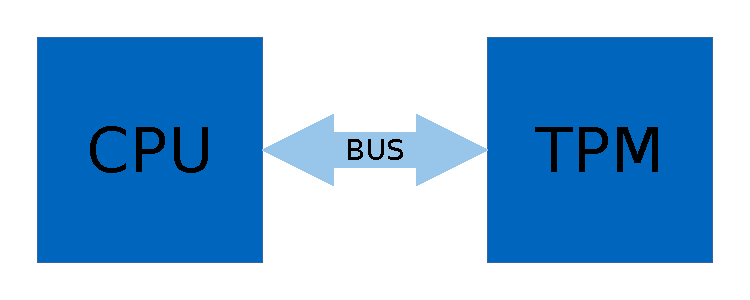
\includegraphics[width=\linewidth]{figures/dTPM.pdf}
      \caption{Discrete TPM} \label{fig:dtpm}
    \end{subfigure}%
    \hspace*{\fill}   % maximize separation between the subfigures
    \begin{subfigure}{0.49\textwidth}
      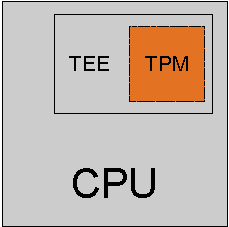
\includegraphics[width=\linewidth]{figures/fTPM.pdf}
      \caption{Firmware TPM} \label{fig:ftpm}
    \end{subfigure}%

    \begin{subfigure}{0.49\textwidth}
      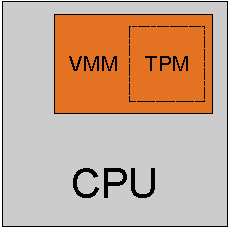
\includegraphics[width=\linewidth]{figures/vTPM.pdf}
      \caption{Virtual TPM} \label{fig:vtpm}
    \end{subfigure}%
  
  \caption{Schematic illustration of the different TPM types. Blue: Hardware, Orange: Software.} \label{fig:tpm_types}
  \end{figure}

There are three types of TPMs. They all offer the same functionality, but with different security guarantees and performance characteristics.

\subsection{Discrete TPM}

This is the classical form of a TPM. It is a dedicated piece of hardware, connected to the CPU via a bus. It is designed and manufactured to be highly temper-resistant against hardware attacks.
The TPM specifications \cite{tpm, tcgPcClient} do not demand a specific bus system, however, they define the interfaces between the TPM and the following bus systems: LPC, I\textsuperscript{2}C, and SPI.

The well-known 'TPM Reset Attack' was independently described in \cite{kauerBernhard,sparks2007}. It requires minimal hardware, precisely only a wire connecting the reset line of the LPC bus \cite{lpc} to ground. This results in a reset signal for the TPM, yielding predictable values for the \ac{PCR} registers, i.e., 0. This allows an attacker to replay the measurement log of a benign boot process to achieve valid \ac{PCR} values, even though a modified chain has been booted.
Since TPM 1.2, TCG provides a mitigation specification for this reset attack \cite{tcgResetFix}, requiring the BIOS to overwrite sensitive data after each unexpected reset, preventing an attacker to gain a valid measurement log.
% TODO: That's claimed by Winter2013 but that the mitigation works because the attacker cannot gain a valid measurement log is from me. But is measurement log really sensitive? Otherwise I'm not sure how the mitigation prevents the attack, since the spec only changes the behavior of the platform on reset, not the TPM on reset. And with the upper described attack, only the TPM is reset.
However, this mitigation is still vulnerable to cold boot attacks \cite{Halderman2009, Winter2013}.

Winter and Dietrich \cite{Winter2013} demonstrate a bus modification attack at TPMs integrated with the LPC bus or the I\textsuperscript{2}C bus.
Their approach, labeled 'Active LPC frame hijacking', allows them to "lift" commands to a higher locality than the one they were originally sent with. This allows them to evolve the 'TPM Reset attack' from being only usable for S-RTM, to also D-RTM systems.
They also introduce a new approach of circumventing the TPM's measurement feature. Instead of resetting the TPM as previously described \cite{kauerBernhard,sparks2007}, they reset the main device, i.e., the users' device like a desktop PC while preventing the TPM from receiving the reset signal. This keeps the state of the TPM, e.g., the valid \ac{PCR} values of the previous boot procedure, and the attacker can hijack the boot procedure triggered by the platform's reset and boot a malicious operating system or firmware, while the TPM still stores the old and valid PCRs. While its conceptually easier since the attacker does not need to know the measurement log since the valid \ac{PCR} values are already in-place, it requires active manipulation of bus transmissions to shield the TPM from the reset signal.

A passive sniffing attack is shown in \cite{Kursawe2005AnalyzingTP}. It is applicable to TPM 1.1 connected to an LPC bus. They observed that the data of some operations like unsealing are transmitted via the bus in plain text. Since TPM 1.2, however, the modules no longer send sensitive data unencrypted \cite{Winter2013}.

That invasive hardware attacks against dTPMs are possible was already proven by Tarnovsky in 2010 \cite{tarnovsky}. However, this requires a lot of time, knowledge and resources, i.e., hardware and money.


\subsection{Firmware TPM}

As seen in the previous section, the bus between the CPU and a TPM is the biggest attack vector. An fTPM circumvents this by being directly executed within the CPU, revealing no easily accessible bus.

\subsection{Virtual TPM}

% Confidential Computing approaches (Fraunhofer paper), our solution could be a use-case for that

% Provided by hypervisor (not necessarily, I read a paper which does not need to trust hypervisor. Don't remember what provides it.)


\section{Secure Boot and Measured Boot}

Secure boot is a concept of UEFI doing local attestation of components directly at boot-time. Based on signatures of next-to-boot components. It cancels the boot process as soon as deviations are detected. Binaries of components are first signed and then, deployed universally. Hence, binaries are not bound to the platform and can be considered portable in this context.

Measured Boot is a concept that is often implemented in interplay with a TPM. Measured Boot allows remote attestation to a later time. Uses sealing functionality of TPMs, therefore, bound to the exact platform.

Both technologies are often used in conjunction.

% !TeX root = ../main.tex
% Add the above to each chapter to make compiling the PDF easier in some editors.

\chapter{Related Work}\label{chapter:related_work}

In this chapter we provide a collection of scientific work that relates to this thesis.
For each, we provide a brief overview and how they are connected to our work.

\section{Attacks on TPMs}

Generally, attacks on \acp{TPM} target one of two goals.
Either to decouple the host system's actual state and the state measured by the \ac{TPM}, or to reveal secrets stored on the TPM\@.


% Attacks on \acp{dTPM} are relevant as they motivate \acp{fTPM}.
% We also introduce attacks on \acp{fTPM} to show that updates and measuring the exact version of them are important to understand which known vulnerabilities are patched and which are not.

% \subsection{\Acl{dTPM}}

\paragraph{\Acl{dTPM}}

The `TPM Reset Attack' on TPM~1.1 is described independently in~\cite{kauerBernhard,sparks2007}, whereby the state of the host computer and the TPM are decoupled.
It requires minimal hardware, precisely only a wire connecting the reset line of the LPC bus~\cite{lpc} to ground.
The TPM understands this as a reset signal, yielding predictable values for the \ac{PCR} registers.
This allows an attacker to perform a boot process with malicious components, later resetting the \ac{PCR} values to a known value with the reset attack, and then replay the measurements of a benign boot process.
This not only spoofs the attestation process, but also allows the attacker to access secrets stored on the TPM, which is sealed to the benign state of the host machine.
\Ac{TCG} mitigated this problem by introducing localities with TPM~1.2 which restrict the extension of specific \acp{PCR} to special hardware modes that are no longer accessible in the later boot process~\cite{tpmResetMitigation}.

Winter and Dietrich~\cite{Winter2013} circumvent this counter measurement with an attack on \acp{dTPM} integrated with the LPC bus or the I\textsuperscript{2}C bus.
Their approach---labeled `Active LPC frame hijacking'---allows them to ``lift'' commands to a higher locality than the one they were originally sent with.
% This allows them to evolve the `TPM Reset attack' from being only usable for \ac{SRTM}, to also \ac{DRTM} systems.
They also introduce a new approach to disconnect the \ac{TPM}'s measured state and the systems actual state.
Vice versa to the `TPM Reset Attack', they reset the main device, e.g., a personal computer, while preventing the TPM from receiving the reset signal.
This keeps the benign measurements stored by the TPM, while the attacker can compromise the newly booting system without being measured.
% While this is conceptually easier since the attacker does not need to know the measurement log since the benign \ac{PCR} values are already in-place, 
However, it requires active manipulation of bus transmissions to shield the \ac{TPM} from the reset signal.
The original work is from 2013 and therefore focuses on TPM~1.2.
Despite only having access to TPM~2.0 emulators in 2015, Winter mentions in his master's thesis that initial tests indicate that these attacks also apply to TPM~2.0.
To the best of our knowledge, this is the only statement done about these attacks for TPM~2.0.


% A passive sniffing attack is shown in~\cite{Kursawe2005AnalyzingTP}.
% It is applicable to TPM~1.1 connected to an LPC bus.
% They observed that the data of some operations like unsealing are transmitted via the bus in plaintext.
% Since TPM~1.2 the modules no longer send sensitive data unencrypted~\cite{Winter2013}.

% That invasive hardware attacks against \acp{dTPM} are possible was already shown by Tarnovsky in 2010~\cite{tarnovsky}.
% Nevertheless, this requires a lot of time, knowledge and resources, i.e., hardware and money.

% \subsection{\Acl{fTPM}}
\paragraph{\Acl{fTPM}}

As seen in the previous section, the bus between the CPU and a \ac{dTPM} is a typical attack vector throughout their history.
An \ac{fTPM} circumvents this by being directly executed by the CPU within a \ac{TEE}, revealing no easily accessible bus.

Despite that, there are also attacks against \acp{fTPM}.
Moghimi et al.~\cite{Moghimi2019} demonstrate a time-based side-channel attack.
It applies to Intel's \ac{fTPM} before the corresponding software patch in November 2019, and allows an attacker to recover 256-bit private keys for ECDSA and ECSchnorr signatures.
% STM published a solution, but this involves a hardware update and not just a software update.

Seunghun Han et al.~\cite{aBadDream} report two attacks on \acp{TPM} to reset the PCR registers.
The first targets a gray area in the power management section of the TPM~2.0 specification.
If the host platform goes into sleep mode, it can send a command to the TPM demanding it to store its current state including its PCRs in its non-volatile random access memory.
When the host platform wakes up again, it can request that the saved state be restored with a corresponding command.
Nonetheless, the specification lacks a concrete description of the behavior if the TPM has not saved any state before going to sleep, but still receives the command to restore its saved state when waking up.
It merely states that the TPM implementation is expected ``to take corrective action.''
Hence, some implementations simply reset the TPM which resets the \acp{PCR} as well, which also applies to the latest version of the TPM specification at the time of writing~\cite{tpm20}.
Their second attack targets an \ac{fTPM} running with Intel's Trusted Execution Technology.
They exploit that some mutable function pointers are not measured in its measuring boot environment.

Jacob et al.~\cite{Jacob2023} target proprietary AMD fTPMs by attacking their \ac{TEE}, namely the AMD Secure Processor~(AMD-SP).
Thereby, they can expose the full internal state of the \ac{fTPM} bypassing any authentication mechanisms.
To do so, they leak the secret key from the BIOS flash chip which is used to derive the encryption and signature keys for the \acp{fTPM} non-volatile data.
They achieve this by using a voltage fault injection that bypasses the authenticity check in the host's boot process and allows them to boot their own firmware component that leaks the required information.

Cohen from the Google Cloud Security team also targets AMD's fTPM running with the AMD-SP~\cite{cohen}.
They store a maliciously crafted payload---a certificate---on the \ac{fTPM} and trigger a function with a stack-based overflow error that accesses this payload, giving them full control over the program counter.
According to the author, this bug is limited to vendors that diverge from the \ac{TPM} specification, as this issue does not appear in \ac{TCG}'s reference code.

These attacks on \acp{fTPM} show that they need to be updatable to respond to the disclosure of future vulnerabilities.
They should also be measured to understand which known vulnerabilities are patched and which are not.

\section{Hardening of TPMs}

In the following, we describe defense mechanisms for fTPMs that can be seen as complementary to our approach.
They all have in common that they offer no way for a third party to ensure that the hardened fTPM is actually running on the device under test, which is exactly what our work aims to cover.

\subsection{Firmware TPMs}

One approach is to formally verify the code of fTPMs towards specific security properties.
Mukhamedov et al.~\cite{Mukhamedov2013} write portions of the TPM~1.2 code in a functional programming language---namely F\texttt{\#}---that enables automatic verification.

Raj et al.~\cite{Raj2015} call for hardware entropy for a secure \ac{fTPM} implementation, but do not elaborate on how this can be achieved.
Kim and Kim~\cite{Kim2019} propose an abstraction layer on top of an \ac{fTPM} and a \ac{dTPM}---the hybrid TPM~(hTPM), which enables switching between the hardware and software module as required.
They aim to combine their advantages, e.g., by making the dTPM the source for the hardware entropy of the fTPM\@.
In addition, the hTPM performs significantly better in software mode than in hardware mode due to the use of modern CPU features.
But for all that this comes at the cost of increasing complexity.

In contrast, Gross et al.~\cite{Gross2021} propose backing an \ac{fTPM} with hardware without requiring a \ac{dTPM}.
For that, they provide cryptographic and entropy support through hardware.
This inherits the downsides of \acp{fTPM} which are not related to a lack of hardware, but to the nature of software.
For example, their \ac{fTPM} is still started later in the boot chain than a \ac{dTPM}, which is not the case for an hTPM\@.
Despite that, it is easier to update than hTPM since the lack of a dTPM, and the overall design is simpler.

\subsection{Virtual TPMs}

% Due to the increasing popularity of cloud computing, the research of vTPMs focuses less on specific attacks, and more on reducing the trusted computing base, i.e., privacy-focused.
The initially proposed design of virtual \acp{TPM} requires the operating system and the hypervisor to be trusted~\cite{268868}.

Wang et al.~\cite{Wang2019} bring the vTPM into the \ac{TEE}, namely Intel SGX, essentially creating an fTPM and vTPM hybrid.
They launch each vTPM in a private hardware-protected enclave.
This reduces the required trust into to the individual enclaves and SGX itself, enabling the host operating system and hypervisor to be untrusted.

Pecholt and Wessel~\cite{Pecholt2022} describe a design named CoCoTPM where the hypervisor and the host's operating system do not need to be trusted as well.
This is realized by establishing an integrity-protected secure channel with end-to-end encryption between the driver in the VM and the software TPM on the host.

Stateless ephemeral vTPMs~\cite{Narayanan2023} eliminate the need of manually establishing a secure channel by leveraging the confidential VM memory encryption provided by AMD's SEV-SNP, a variant of AMD secure encrypted virtualization~(SEV) technology.
Ephemeral vTPMs support the remote attestation of virtual machines.
On the other hand, they intentionally do not support persistent storage to preclude exfiltration attacks on the TPM's data-at-rest, which has the disadvantage that persistent keys or nonvolatile indexes cannot be stored.

\section{Remote attestation schemes}

% Other defense concepts

% Linux attested with DICE directly instead of TPM?
% Probable disadvantage: not TPMs common interfaces
% and DICE certificate chain size grows linearly, PCR register size is fixed. However, event log also grows linearly, but less data (less information, but less storage overhead)

% https://www.eurecom.fr/fr/publication/3536/download/rs-publi-3536.pdf
The SMART attestation mechanism proposed by Defrawy et al.~\cite{EURECOM+3536} establishes a \ac{DRTM}.
Since their overall approach is similar to \ac{DICE}, they only hardware requirement is a ROM containing a key (corresponding to DICE's \ac{UDS}), and that can only be accessed by SMART\@.
Their secret key is directly used to sign attestation data, while for \ac{DICE} the \ac{UDS} acts as entropy to derive individual secrets from for each firmware component.
SMART thus provides a \ac{DRTM} in contrast to the \ac{SRTM} provided by \ac{DICE} enabling the remote attestation of an \ac{fTPM}.
However, it does not allow data to be bound to the identity of a firmware component.

\ac{TCG} offers an adaption of \ac{DICE} with symmetric cryptography which conducts implicit attestation~\cite{dice-symmetric-arch}.
There, the final symmetric key---also called alias key here---derived from the compound identity of the whole firmware and its UDS represent the prover's identity, without propagating the individual identities of each firmware layer like the \acp{TCI} do.
If this alias key is leaked, trust into the system breaks unrecoverable since the same key is generated on each boot.
DICE+ proposed by Jia et al.~\cite{Jia2020} solves this by equipping the prover with a monotonic counter, which is incremented on each reboot.
This counter influences the alias key, which consequently alters the attestation result derived from it after each reboot as well.
The verifier can calculate the expected attestation data by combining the used counter value, the UDS, and the expected firmware identity.
DICE+ assumes that there is only a single verifier who knows the received values of all previously conducted remote attestations, and can therefore detect replay attacks.
The verifier and the prover must have shared secrets due to the nature of attestation based on symmetric cryptography.
DICE+ shares the prover's UDS and also the initial monotonic counter with the verifier during the prover's provisioning in an out-of-band manner.
While their approach is practical for low-end devices that are not capable of asymmetric cryptography, we are targeting machines with a processor with a \ac{TEE}, which implies a certain amount of computation power.
We also do not want to require pre-shared secrets between the verifier and the prover.
In addition, the TPM's infrastructure demands asymmetric cryptography for signing the EK certificate, and the monotonic counter would change the TPM's identity on each reboot, effectively hindering the binding of the fTPM's data to its identity.
Hence, we use DICE with asymmetric cryptography instead.

% They claim it is implicit, but I believe they have another understanding of implicit and explicit as what I use in this thesis (the one from the DICE spec). So I just leave it, as it is only confusing and not of great importance.
Bravi, Sisinni, and Lioy~\cite{Bravi2023} propose an attestation system with DICE for IoT devices running with the RISC-V ISA without TEE\@.
While we combine DICE with the TPM infrastructure, they combine it with the Manufacturer Usage Description (MUD).
MUD allows a device to signal to the network what kind of access and network functionality it requires for further access control~\cite{Lear2019}.
It also explains how DICE can be implemented with the novel RISC-V technology Physical Memory Protection~(PMP).
Their design is orthogonal to ours, and they are compatible.
This is because we are not limited to a specific DICE implementation and their support for MUD is integrated via an X.509 certificate extension that can trivially be added to our system as well.

\section{DICE implementation}

Jäger, Petri, and Fuchs~\cite{Jaeger2017} describe how the remote attestation procedure described in the DICE specification can be put into practice by discussing implementation options.
Thereby they complement our work by evaluating how to implement \ac{DICE}\@.
Jäger and Petri continue their work later~\cite{Jaeger2020} because they observed a limitation in their initial implementation, allowing to jump into \ac{DICE} code possibly leaking the \ac{UDS}.
Lorych and Jäger carried on exploring the design space of DICE~\cite{Lorych2022} later on.
As with SMART, the goal of all these publications is not to attest an \ac{fTPM} and therefore do not describe how to combine the infrastructure of DICE and \acp{fTPM}.

Just as we presented a paper proposing a formally verified \ac{fTPM} implementation, Tao et al.~\cite{272306} propose a formally verified \ac{DICE} implementation called DICE\( ^* \).
They focus on the software side of the first DICE layer and are agnostic to the actual hardware used.
Therefore, it can be used together with the hardware designs from the previously listed works.

% TEE attestation

% M{\'{e}}n{\'{e}}trey et al.~\cite{Menetrey2022} discuss attestation mechanisms for \acp{TEE}.
% Our \ac{fTPM} is also running in a \ac{TEE}, and can thereby be attested with this approach.
% However, it assumes that the entire TEE is trusted


% Attacks which we would avoid (e.g., exchange/spoof EKcert)


% https://dl.acm.org/doi/pdf/10.1145/3600160.3600171
% This requires trusting the measurement root of trust (there TPM, AMD SEV-SNP or Arm PSA Attestation Token), but also need to trust the operator to provide benign reference values.
% Or not if the operator of the trust anchor is the same as the operator of the device. Or the trust anchor and the reference values root in the operator. Operator needs to sign (and beforehand verify) not only the trust anchor, but also reference values (high burden).
% The paper also only mentions hardware trust anchors, no fTPMs. Could be used in conjunction. I believe our cert chain up to the fTPM would need to be provided within the Attestation Report, but system independent, i.e., would need to be independent of the concrete technology (here DICE). Not sure if that's possible.

% https://www.amd.com/en/processors/amd-secure-encrypted-virtualization
% For virtual machines
% Auch https://arxiv.org/pdf/2204.06790.pdf
% 3.5

% https://ieeexplore.ieee.org/abstract/document/9292371

% https://netsec.ethz.ch/publications/papers/mccune_parno_perrig_reiter_isozaki_eurosys08.pdf


\appendix{}

\microtypesetup{protrusion=false}

\addchap{Abbreviations}
\begin{acronym}
	\itemsep-.25\baselineskip
	\acro{TUM}[TUM]{Technical University of Munich}
	\acro{TPM}[TPM]{Trusted Platform Module}
	\acro{TEE}[TEE]{Trusted execution environment}
	\acro{REE}[REE]{Rich execution environment}
	\acro{HSM}[HSM]{Hardware Security Module}
	\acro{PCR}[PCR]{Platform Configuration Register}
	\acro{TCG}[TCG]{Trusted Computing Group}
\end{acronym}

\listoffigures{}
\listoftables{}
\microtypesetup{protrusion=true}
\printbibliography{}

\end{document}
